%!TEX root = JournalChapter1.tex
\subsection{Dimensions Interaction.}

To further our analysis in the structure of microblog documents we studied how the different dimensions interact with each other. Apart from the presence of the dimensions above discussed, we believe that the order in which they appear, and the interactions between them are also important. In fact, there are several documents on the web \footnote{http://blog.hubspot.com/marketing/tweet-formulas-to-get-you-started-on-twitter} which are meant to assist in writing the perfect tweet to grab the attention of readers.


\subsubsection{State Machine Structure}
To properly model such interactions is no simple task. In our study we utilised all documents in the relevance judgements from the Tweets 2013 collection as our training set. Each tweet is tokenised, and each token is categorised as representing each of the ``text'', ``hashtag'', ``mention'' and ``url'' dimensions, with the help of simple regular expressions matching. Moreover we quantify the frequency that a dimension is followed by another one. For example, we count the number of times when text leads to a hashtag, or a mention leads to a url. The frequencies of each dimensions leading to another dimension of the microblog documents are then utilised to build a simple state machine (or automata). Figure \ref{automataexample} shows an example, denoting how state 1, can transition to other states, such as state 2, with the probabilities stated above the arrows \footnote{ Notice that all transition probabilities for a node add up to 1.}. 



\begin{figure}[h!]
\vspace{0.5cm}
\hspace{3.5cm}
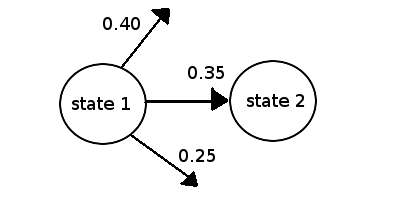
\includegraphics[scale=0.6]{example.png}
\caption{State machine example.}
\label{automataexample}
\vspace{0.5cm}
\end{figure}



Figures \ref{relevantautomata} and \ref{nonrelevantautomata} show state machines for both relevant and non relevant documents respectively. Both these figures contain a node to represent each of the dimensions studied in previous sections. Additionally they contain a ``\textbf{start}'' and ``\textbf{end}'' nodes, to denote the beginning and ending of the microblog document. Consequently, every existing tweet can be characterised by a particular path from the \textbf{start} to the \textbf{end}.



While both figures look very similar, there are some differences that are worth noting. Firstly, looking at the transition from mentions to the end of the document, we can see that the probability for relevant documents is more than double (+21\%) than that for non-relevant documents. This means that relevant documents are more likely to finish mention than non-relevant microblogs.

Likewise the probability of ending a relevant document with a token of text is 12\% less than for non-relevant documents. Moreover the chance of transitioning from a text token to a url token is 13\% higher for relevant documents compared to non-relevant microblogs. Finally the chances to start a document with a mention is half ( 6\% less) for relevant documents with respect to non-relevant ones.

In order to test whether we can use this evidence for producing better rankings, we devised our \textbf{``State''} approach. The State approach is a re-ranking method that linearly combines the score given by any retrieval method with the aggregation of probabilities from start to end nodes w.r.t a microblog's structure.

%!TEX root = main.tex
\begin{figure}
\begin{smaller}

        \begin{subfigure}[b]{\textwidth}
        \vspace{-2.5cm}
        \hspace{-1.5cm}
        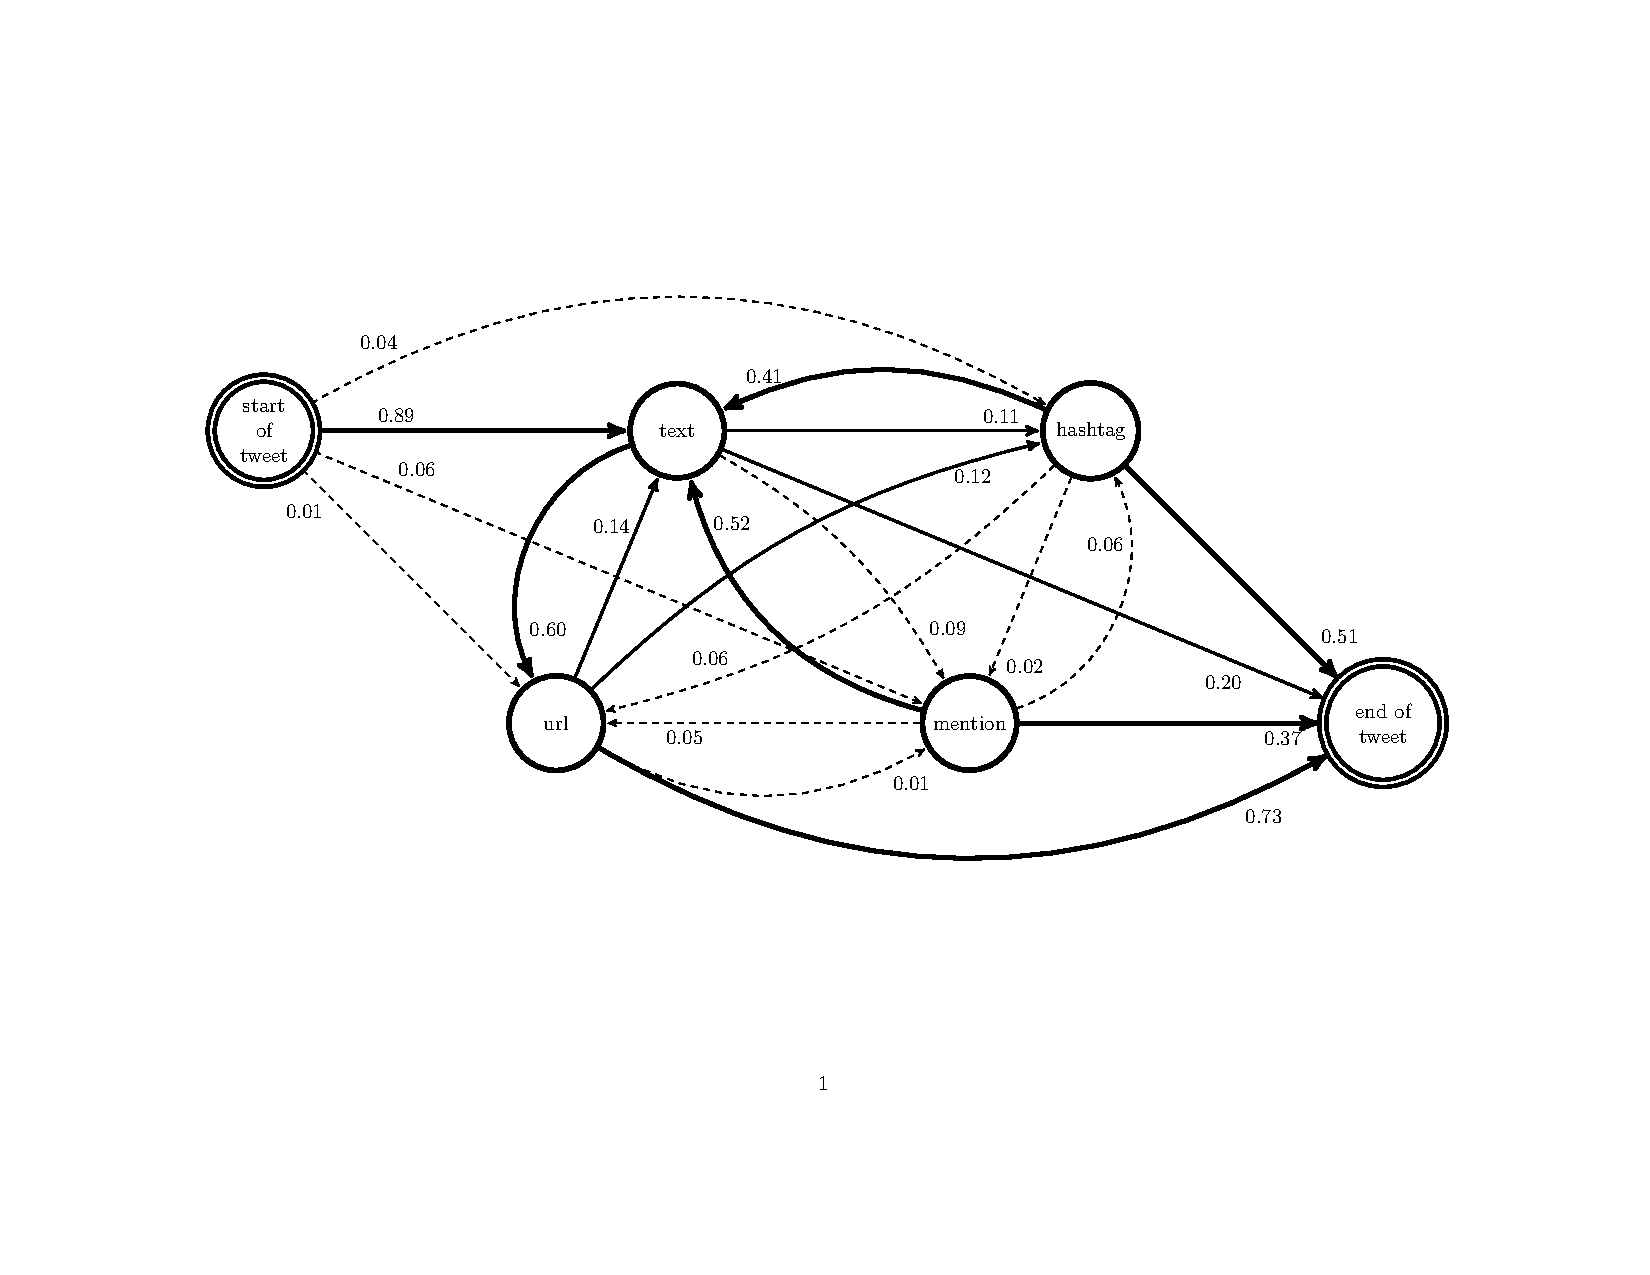
\includegraphics[width=17cm]{automatarelevant.pdf}	 
        \vspace{-4cm}  
        \caption{Relevant documents}
        
        \label{relevantautomata}
        \end{subfigure}
		
        \begin{subfigure}[b]{\textwidth}
        \vspace{-2.5cm}
        \hspace{-1.5cm}
        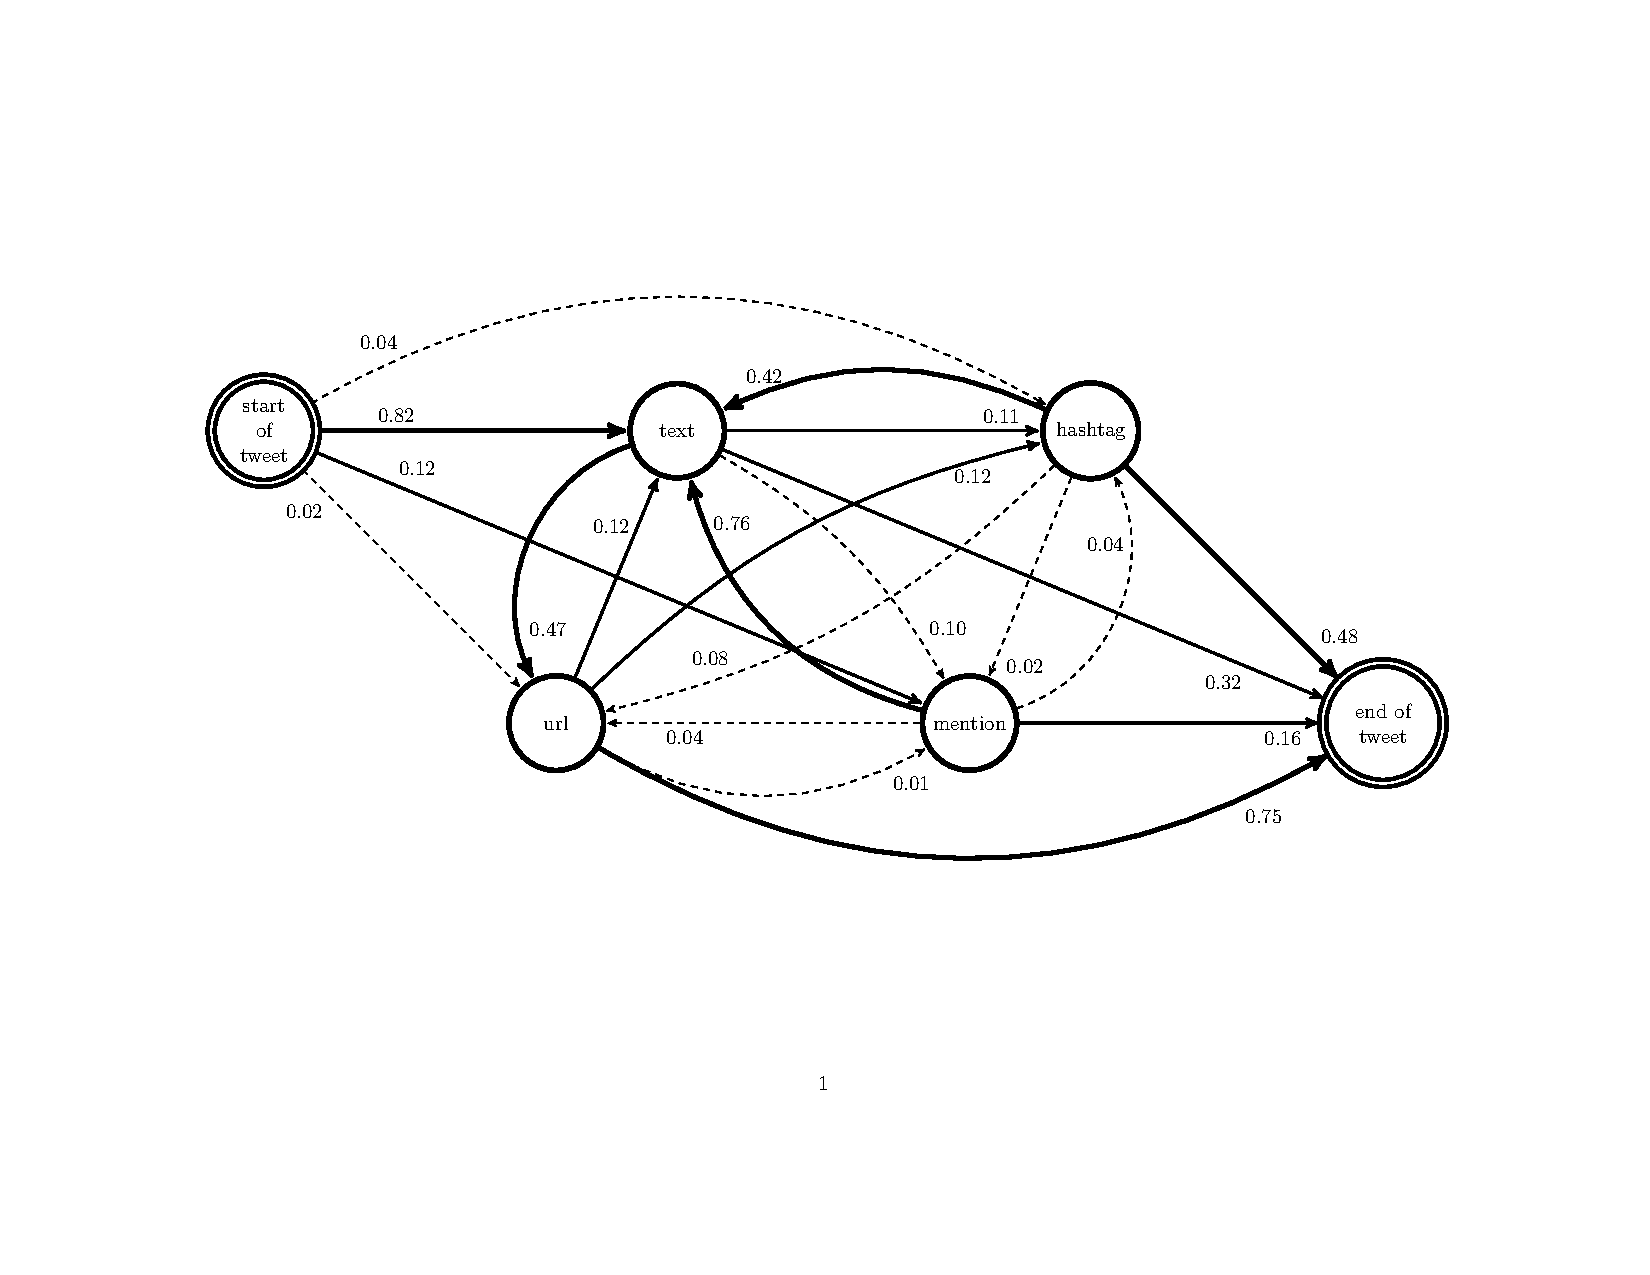
\includegraphics[width=17cm]{automatanonrelevant.pdf}
        \vspace{-4cm}
        \caption{Non-Relevant documents}
        \label{nonrelevantautomata}
        \end{subfigure}      
\end{smaller}

\caption{Tweet automatas for the 2013 collection}
\label{automatas}
\end{figure}




As an example, consider the following tweet: \textit{``Astronomers discover ancient system with five small planets. Details: http://go.nasa.gov/1wCpkJn  @NASAKepler''}. Following the approach described above, we can infer the following structure: ``\([start]->[text]->[url]->[mention]->[end]\)''. If we take the automata for relevant documents (Figure \ref{relevantautomata}) as the source of probabilities it would produce the score: \(0.89 + 0.60 + 0.01 + 0.37 = 1.87\). 



The ``State'' score therefore is given by the following equation:



\begin{equation}
\begin{split}
   State(D,Q) = (1-\alpha)P(q \subset D|Q) \\
   +\alpha * (R\_Score(D) - NR\_Score(D)),
\end{split}
\end{equation}\\



where \(R\_Score(D)\) and \(NR\_Score(D)\) are the scores computed by traversing the automatas in Figures \ref{relevantautomata} and \ref{nonrelevantautomata} respectively and \(\alpha\) is a weighting factor which balances the linear combination. Notice the subtraction of the score given by the automata based on non-relevant documents with respect to the score based on relevant documents. The intuition is that, we want documents that agree with the structure observed for relevant documents, whilst diverging from that of non-relevant documents.







\begin{table}
	\caption{Experimental results for the State retrieval method on the 2011 and 2012 collections. (* \(p<0.05\) and \(\dagger\) \(p<0.01\))}
	\centering
		\begin{tabular}{c|c|c|c|c|c|c}
			& P@5 & P@10 & P@15 & P@20 & P@30 & MAP \\
			\hline
			Baseline & 0.458 & 0.432 & 0.399 & 0.382 & 0.362 & 0.109 \\
			\hline
			State\_0.02 & 0.451 & 0.434 & 0.408 & 0.396* & 0.358  & 0.108 \\
			State\_0.03 & 0.475 & 0.452\(\dagger\) & 0.414* & 0.395* & 0.362  & 0.108  \\
			State\_0.05 & 0.478 & \textbf{0.469\(\dagger\)} & \textbf{0.428\(\dagger\)} & 0.395* & \textbf{0.369}  &\textbf{ 0.110} \\
			State\_0.07 & \textbf{0.481} & 0.454 & 0.416 & \textbf{0.398*} & 0.361 & 0.107 \\
			State\_0.10 & 0.458 & 0.424 & 0.397 & 0.377 & 0.349  & 0.103  \\
			\hline
		\end{tabular} 

	\label{AutomataResults}
	\vspace{0.5cm}
\end{table}





Table \ref{AutomataResults} shows the retrieval results for our re-ranking approach over the 2011 and 2012 collections. P@5 to P@30 represents Precision at the different cut-off points, whereas MAP denotes Mean Average Precision at cut-off 30. The first column contains the model being evaluated. Baseline represents a simple retrieval run using DFR only for ranking, whereas ``State\_n'' contain the results for our ``State'' approach with different values of \(\alpha\). 



As we can observe, retrieval effectiveness is improved significantly for a number of measures. Specifically the ``State\_0.05'' configuration achieved a \(p\) value below 0.01 for both P@10 and P@15. We can see how the most prominent improvements are achieved at the top cut-off points. This result suggests that taking into consideration the structure of documents, helps in bringing more relevant documents to the very first few documents, which is a highly desirable product due to the fast-paced environment that is microblog search.



%\subsubsection{Tree Structures}
%Whilst the state machine managed to effectively capture the tweets structure as evidenced by the statistically significantly improved retrieval performance reported in \cite{rodriguezPerez}, there are a number of issues. By design the state machine model is only aware of how \textbf{A} can transition to \textbf{B}, and previous transitions have no effect in the model itself. In other words, the fact that text following a mention is in the middle of the tweet or near the end, has no effect in the edge values. Furthermore, the values on an edge between \textbf{B} and \textbf{C} are not affected by a previous transition \textbf{A} to \textbf{B}.
%
%This limitation motivated the design of \textbf{TwTree} short for ``Tweet Tree''. As the name suggests, we decided to encode the structure of tweets in a tree-like structure. Our intuition is that by utilising a tree-like structure we may represent such sequences of elements in full, thus achieving a higher level of granularity. 
%
%%Moreover we build a tree for relevant tweets and another for non-relevant tweets. 
%Similarly to the work by \cite{rodriguezPerez} we tokenize the tweets thus decomposing them into their building blocks: text, mentions, hashtags and urls. We then specify the root of the tree and the ``start'' of the tweet. All tweets from either the relevant or non-relevant set are then added to the tree one element at a time in order thus becoming a path from the root of the tree specified as ``start'' and ending in the leaf node specified as ``end''. Every time we add a new tweet to our structure we note the number of times that such structure has occurred as \(t\). Concurrently, we keep the total number of tweets \(T\) that have been employed to build the tree at the root node ``start''.
%
%\begin{figure}[h!]
%\centering
%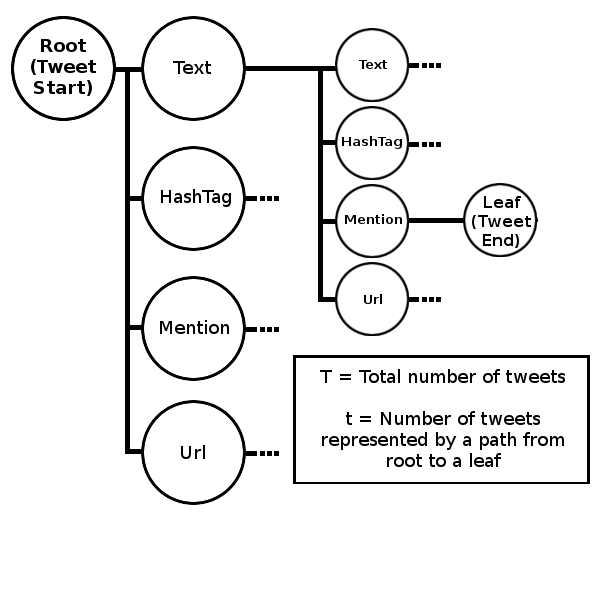
\includegraphics[scale=0.50]{treeStructure.png}
%\caption{Tree structure to represent sets of tweets.}
%\label{treeExample}
%\end{figure}
%
%
%Figure \ref{treeExample} shows a simplified example of such tree structure. Let's assume we have a tweets which structure is defined as: 
%
%\begin{equation}
%[start]->[text]->[mention]->[end]
%\label{sequence}
%\end{equation}
%
%\noindent the score is computed by traversing the tree following the sequence \ref{sequence} and extracting the \(t\) value at the leaf, and dividing by the total number of tweets that have been used to create the model \(T\). Thus the score is simply obtained by \(t/T\) and it represents how common is this structure amongst all the tweets that have been used to form the model. Notice that the score will always be a normalised value between 0 and 1, which simplifies later computations.
%
%Similarly to the state machine based system created by \cite{rodriguezPerez} we will create a tree representing relevant documents and another for non-relevant documents. Consequently we may produce an score from each model R\_TwScore(D) and NR\_TwScored(D) for any given document \(D\). Finally the scores are to be merged as follows:
%
%\begin{equation}
%merge(D) = \frac{R\_TwScore(D)}{R\_TwScore(D) + NR\_TwScore(D)}
%\label{merge}
%\end{equation}
%
%\noindent This equation always returns a value between 0 and 1. The closer the value is to 1 the closer the structure of document \(d\) resembles the relevant set of tweets and vice-versa. As an example consider:
%
%\begin{equation}
%\begin{split}
%R\_TwScore(D)= 0.75 \\
%NR\_TwScore(D) = 0.60
%\end{split}
%\end{equation}
%
%Consequently the score obtained by $merge(D)$ will be 0.55, which means tweet $D$ resembles a bit more the set of relevant tweets than the non-relevant set.
%
%Finally, the score \(TwTree(D)\) is given by its linear combination with a retrieval model \(P(q \subset D|Q)\) as follows:
%
%\begin{equation}
%\begin{split}
%   TwTree(D,Q) = (1-\alpha)P(q \subset D|Q) \\
%   +\alpha * merge(D),
%\end{split}
%\end{equation}\\
%
%
%\noindent{\bf Loose sequence matching. } As an additional note, there is a possibility that a particular sequence may not yet exist within a TwTree model. To address this problem, we perform a loose matching as we consider that returning the score for a closely related structure is better than not returning anything at all. 
%
%As an example, if we look up the following sequence:
%
%\begin{equation}
%[start]->[text]->[mention]->[url]->[text]->[end]
%\end{equation}
%
%but only the following sequence is avaiable: 
%
%\begin{equation}
%[start]->[text]->[mention]->[url]->[end]
%\end{equation}
%
%then the score associated with the later sequence will be returned, and the last text element in the former sequence will be ignored.
%
%%design
%%
%%scores computation 
%%
%%scores merging
%%
%%TreeTweet score linear combination
%
%In the following section we will introduce our experimental setting which precedes our discussions section where we present our findings.
%
%
%
%
%\mentalnote{ADD RESULTS AND DISCUSSION for TREE-STRUCTURE}
%


We can conclude from these experiments that the structure of tweets can be extracted and leveraged to produce better rankings. We can confirm that not only it is the relative space in terms of characters dedicated to each dimension that links to relevance, but also how these dimensions relate to each other within the document.



\subsection{Additional notes}

The simplicity of the state modelling allows for it to be conveniently stored and re-used in real-time. The states are stored as a set of precomputed heuristics which include the dimensions in the transition and its associated probability based on the observed data. The model itself should be updated from time to time to accommodate any shifting in the structuring and style of micro-bloggers.

